\chapter{Introduction \& positionnement de l'étude}

\section{Contexte général}
\subsection{Contexte écologique \& énergétique}
Le monde fait aujourd'hui face à un défi écologique majeur, que l'ONU qualifie de "\textit{menace existentielle directe}" \cite{noauthor_direct_2018}. Le déclin de nombreuses populations animales et végétales est aujourd'hui largement documenté, que ce soit au niveau des insectes \cite{hallmann_more_2017}, des oiseaux \cite{inger_common_2015} \cite{rosenberg_decline_2019} ou encore des espèces d'eau douce \cite{he_global_2019}. D'un point de vue plus anthropocentré, près de 9 millions de décès prématurés par an sont associés à la pollution atmosphérique \cite{burnett_global_2018}, près d'un quart de la population mondiale répartie dans 17 pays est dans une situation de "stress hydrique extrêmement élevé" \cite{kuzma_25_2023}, et environ 30\% de la population mondiale est soumise à des conditions de température et d'humidité mortelles pendant plus de 20 jours par an \cite{mora_global_2017}. Ce constat est actuel et déjà palpable alors que le réchauffement climatique n'est que de l'ordre de 1,1\textdegree C entre 1900 et 2020 \cite{noauthor_ar6_nodate}. Il est également établi que le réchauffement actuel est d'origine anthropique \cite{noauthor_ar5_nodate}, et que ce sont les émissions de gaz à effet de serre, et en particulier de CO2 qui ont l'effet le plus important \cite{noauthor_ar6_nodate}. Une grande partie de ces émissions de gaz à effet de serre vient de la production d'électricité pour le réseau, avec une grande variabilité entre les pays \cite{noauthor_resume_nodate}. Cet aspect, associé au caractère fini des ressources fossiles, a motivé ces dernières décennies le développement de la production d'énergie par des sources renouvelables non directement émettrices \cite{noauthor_shift_nodate}. On retrouve dans ces sources traditionnellement la production hydraulique, photovoltaïque et éolienne. Ces deux dernières sources sont décentralisées par nature, et très dépendantes de l'environnement dans lequel elles se trouvent. Les productions d'énergie photovoltaïque et éolienne sont également majoritairement déployées à des échelles réduites et ont le défaut d'être intermittentes, étant respectivement dépendantes de l'ensoleillement et du vent. Bien que ces sources d'énergie présentent un réel intérêt environnemental, cette intermittence peut compliquer leur intégration au réseau si leur part est prépondérante. Une solution pour pallier ce problème est d'utiliser des moyens de stockage temporaires de l'énergie. À grande échelle, les Stations de Transfert d'Énergie par Pompage (STEP) ont fait leurs preuves \cite{zhao_review_2022}\cite{wang_coordinated_2023} grâce à leur grande capacité, tandis qu'à échelle réduite les batteries \cite{khezri_optimal_2022}\cite{rouholamini_review_2022}, piles à combustible \cite{inci_review_2019}\cite{hossain_advancement_2023}, supercondensateurs \cite{ibrahim_overview_2021}\cite{navarro_present_2021} ou encore volants d'inertie \cite{calero_review_2023}\cite{li_review_2022} peuvent être intéressants, présentant tous des énergies et puissances spécifiques variables pour diverses applications \ref{sto}.
\begin{figure}[h!]
    \centering
    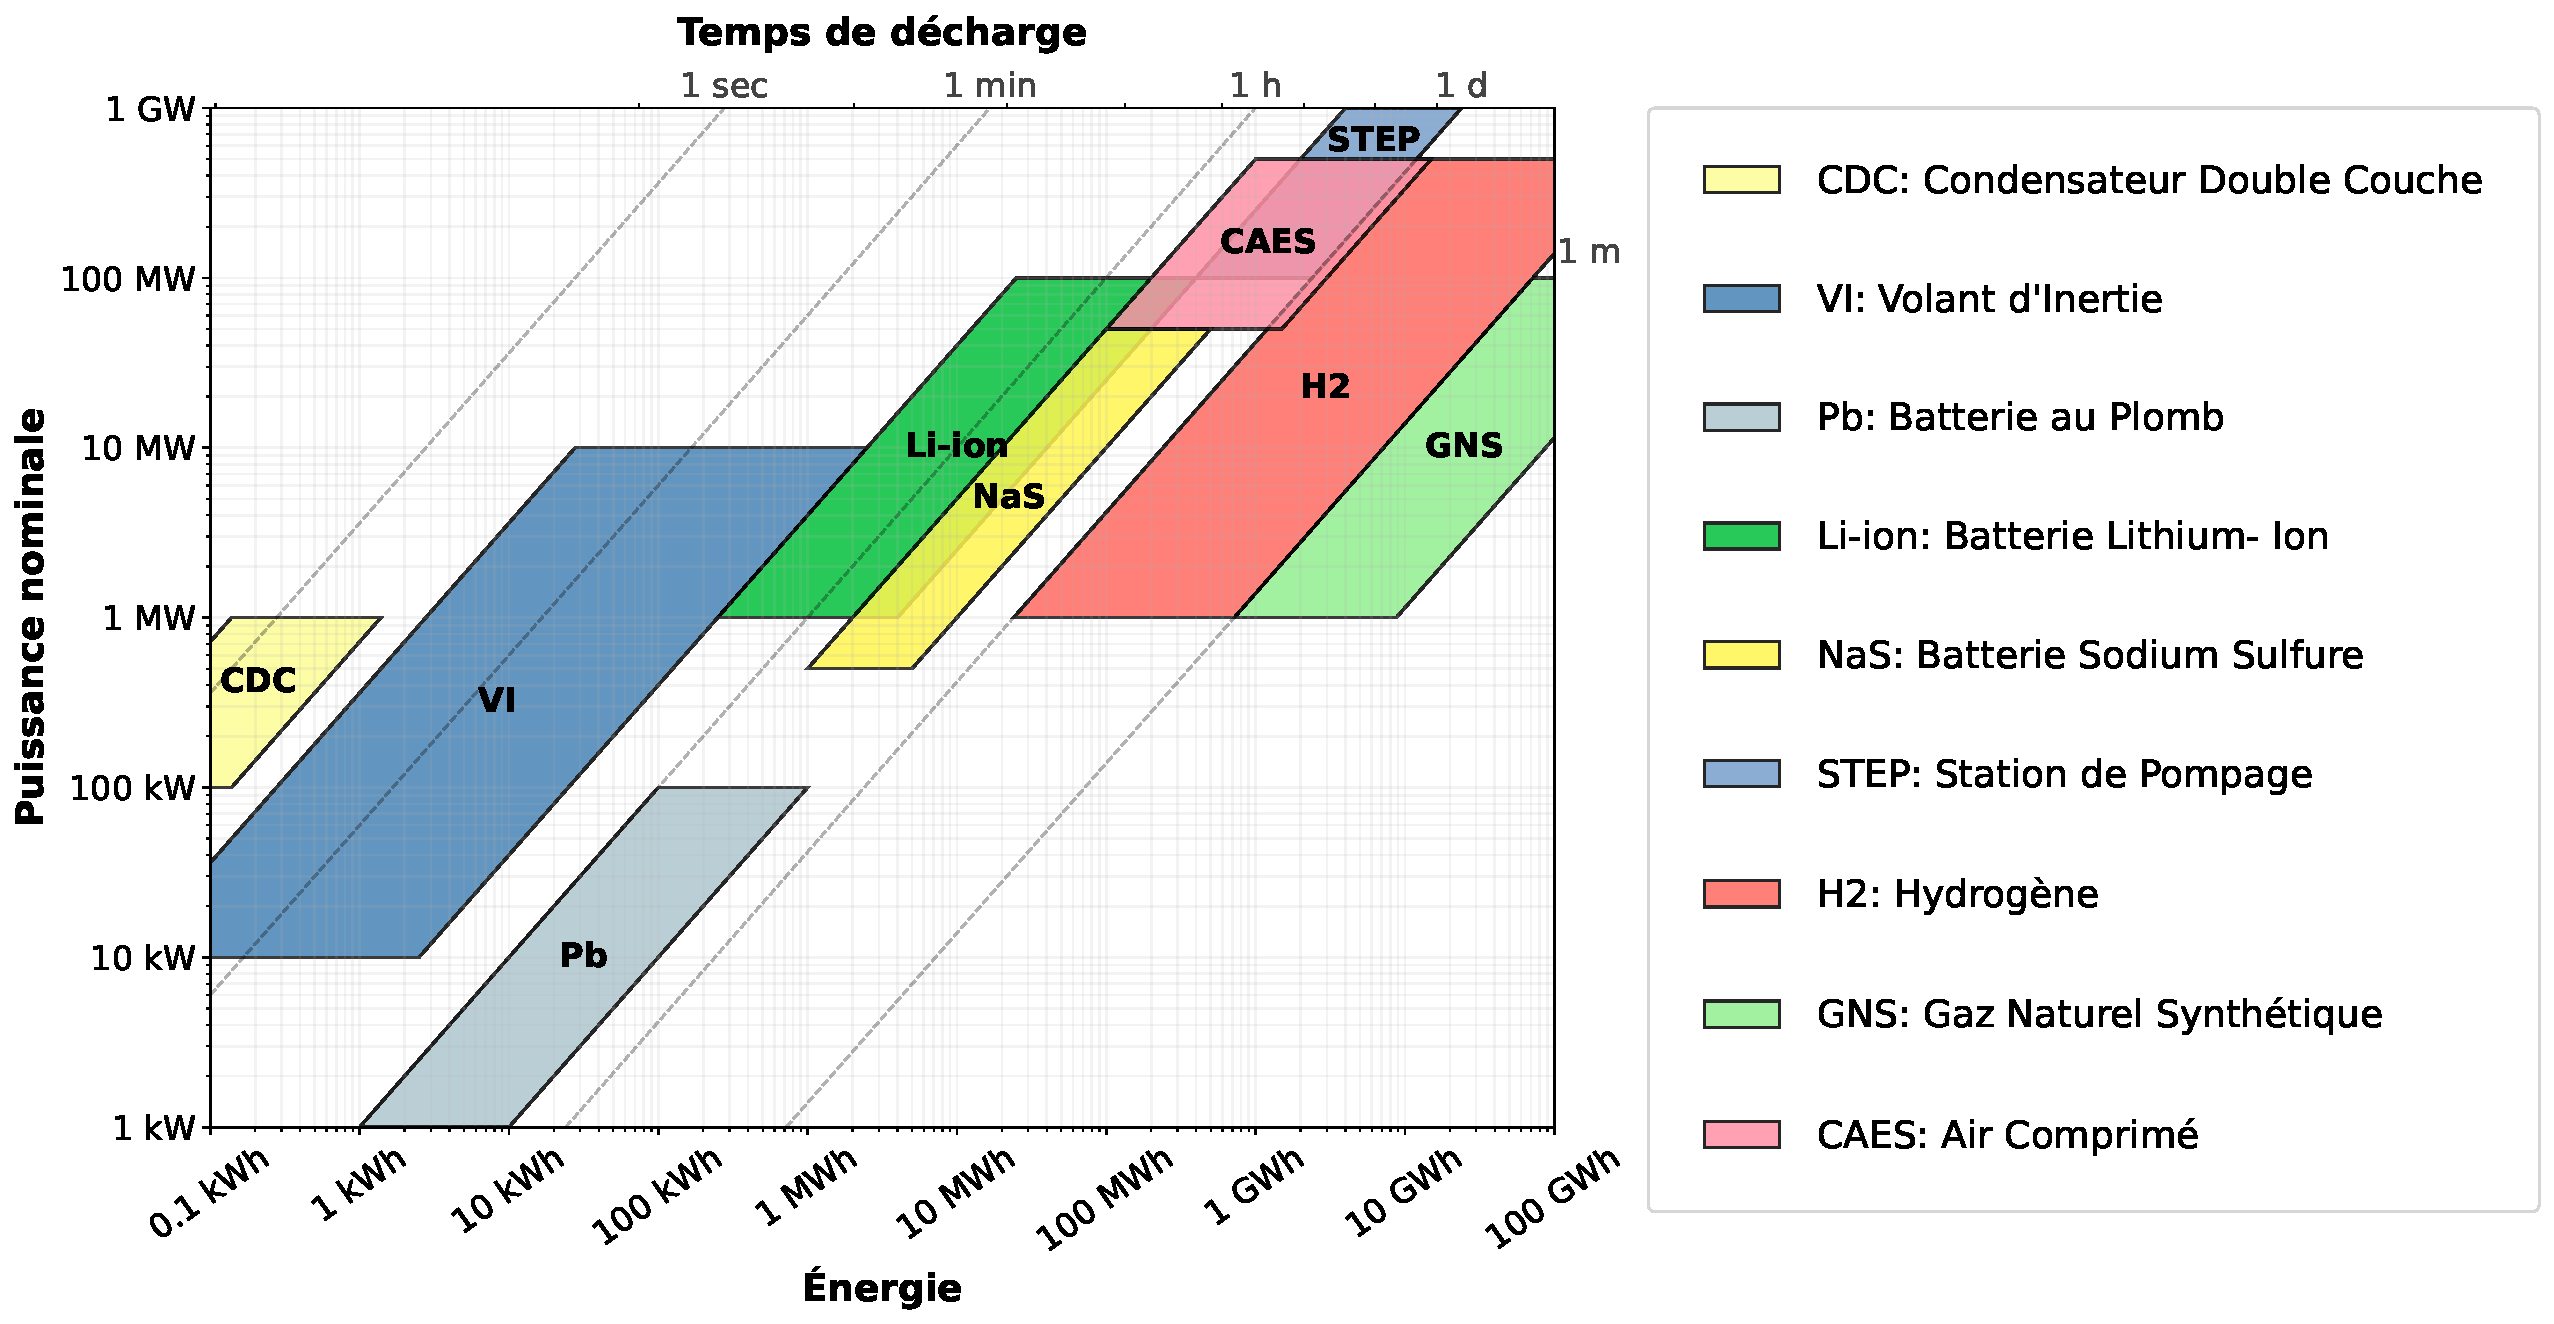
\includegraphics[width=.8\linewidth]{Introduction/Figures/ragone.pdf}
    \caption{Comparaison des caractéristiques des éléments de stockage}
    \label{sto}
\end{figure}
\FloatBarrier
Les réseaux électriques centralisés tels que majoritaires aujourd'hui sont également dépendants de la fiabilité du nombre limité de sources qui les composent. En effet, chaque source étant responsable d'une production importante, n'importe quelle défaillance peut entraîner des répercussions de grande ampleur, et en ce sens des micro-réseaux électriques capables de fonctionner de manière autonome se justifient. En effet, si ces micro-réseaux contiennent leurs propres sources d'énergie suffisantes pour subvenir à leurs besoins, alors ils ne sont plus dépendants de la connexion au réseau principal, augmentant la résilience globale de l'approvisionnement. C'est le cas par exemple dans des installations critiques comme les hôpitaux où le maintien d'une alimentation en électricité est une nécessité. C'est sur ce point et sur la décentralisation par nature des sources d'énergie renouvelable évoquée précédemment que les micro-réseaux trouvent ainsi un intérêt croissant. 

\subsection{Contexte du projet ANR GENIAL}

Cette thèse s'inscrit dans le cadre du projet ANR GENIAL (GEstion d'éNergie d'un mIcro-réseAu à hydrogène résiLient au vieillissement), un projet collaboratif multi-laboratoires d'une durée de 42 mois. Le consortium regroupe plusieurs laboratoires en génie électrique, automatique et sciences humaines et sociales, ainsi qu'un partenaire local (Sidélec, distribution électrique de l'île de La Réunion, France), et s'appuie notamment sur trois doctorants travaillant sur des problématiques complémentaires. L'articulation générale du projet est présentée en fig. \ref{structure_aapg}.

\begin{figure}[h]
    \centering
    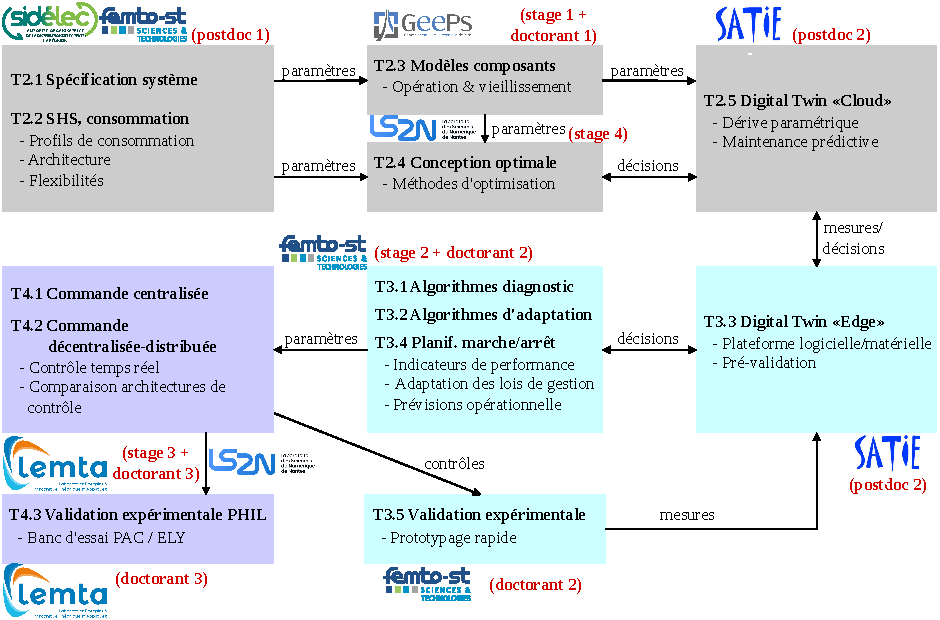
\includegraphics[width=0.8\textwidth]{Introduction/Figures/structure_genial.pdf}
    \caption{Organisation du projet ANR GENIAL }
    \label{structure_aapg}
\end{figure}
\FloatBarrier

Le projet porte sur l'étude d'un micro-réseau électrique continu (DC) couplant des sources renouvelables et une chaîne hydrogène. Le système considéré comprend une production photovoltaïque, une pile à combustible, un électrolyseur, des dispositifs de stockage (batteries et hydrogène) ainsi que des charges électriques (fig. \ref{fig:microgrid_genial}). 

\begin{figure}[h]
    \centering
    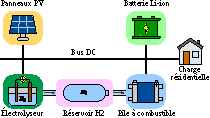
\includegraphics[width=0.8\textwidth]{Introduction/Figures/architecture_v5.pdf}
    \caption{Architecture du micro-réseau hydrogène-énergie étudié }
    \label{fig:microgrid_genial}
\end{figure}
\FloatBarrier

Le cas d'étude considéré dans le projet est un micro-réseau isolé situé à l'îlet de Roche Plate, à La Réunion, destiné à alimenter une douzaine d'usagers. Ce cas d'étude réel constitue un terrain d'expérimentation privilégié pour l'évaluation des approches développées.

Les travaux menés dans le cadre du projet GENIAL portent sur plusieurs problématiques liées à la conception, au pilotage et à la durabilité des micro-réseaux hydrogène. Dans ce cadre, les travaux doctoraux sont structurés autour de trois axes principaux :

\begin{itemize}
    \item \textbf{Dimensionnement optimal du système} : une première thèse vise à développer des outils et méthodes d'optimisation permettant de concevoir un micro-réseau performant en intégrant des critères techniques, économiques et environnementaux, ainsi que les effets du vieillissement des composants sur le long terme.
    
    \item \textbf{Gestion d'énergie résiliente au vieillissement} : celle-ci a pour objectif de développer des stratégies de gestion d'énergie prenant en compte l'état de santé des composants du stockage d'énergie (batteries, pile à combustible, électrolyseur) via des approches de type jumeau numérique et des mécanismes d'adaptation en ligne. L'enjeu est d'améliorer la durabilité du système tout en garantissant ses performances opérationnelles.
    
    \item \textbf{Commande temps réel du micro-réseau} : cette thèse s'intéresse à la conception de lois de commande (centralisées, décentralisées ou distribuées) permettant d'assurer la stabilité dynamique du micro-réseau et une gestion optimale des flux de puissance en temps réel.
\end{itemize}\vspace{0.3cm}

Les travaux présentés dans ce manuscrit s'inscrivent dans la problématique de gestion d'énergie résiliente au vieillissement. Ils apporteront une contribution dans les méthodes permettant d'intégrer des indicateurs de vieillissement dans les stratégies de pilotage, en s'appuyant sur des outils de diagnostic et de pronostic. L'objectif est de proposer une gestion adaptative capable de prendre en compte les évolutions du système au cours de son cycle de vie pour maintenir un équilibre entre performance, robustesse et durabilité.

\section{Présentation du système étudié}
\subsection{Présentation générale des micro-réseaux électriques}
\subsubsection{Définition}
Il convient avant toute chose de définir l'objet d'étude de ce travail. Selon l'\textit{Institute of Electrical and Electronics Engineers (IEEE)}, un micro-réseau électrique peut se définir comme "un groupe de charges interconnectées et de ressources énergétiques distribuées avec des limites électriques clairement définies qui agit comme une entité unique contrôlable par rapport au réseau et peut se connecter et se déconnecter du réseau pour lui permettre de fonctionner à la fois en mode connecté au réseau et en mode isolé" \cite{noauthor_ieee_nodate}. L'entreprise publique de production d'électricité  française \textit{Électricité De France (EDF)} propose une définition plus concise d'un micro-réseau électrique : "Un microgrid est un réseau électrique indépendant, avec ou sans connexion au réseau principal. Sa capacité peut aller de quelques kW à plusieurs dizaines de MW" \cite{noauthor_microgrid_nodate}. 

\subsubsection{Applications}
Les micro-réseaux se distinguent des réseaux traditionnels par leur échelle réduite et une production plus décentralisée. Ils permettent souvent une grande flexibilité dans la gestion de l'énergie, ce qui explique leur utilisation dans de nombreuses applications. On les retrouve notamment beaucoup dans le secteur résidentiel \cite{ali_review_2021}\cite{sabry_compatibility_2020}\cite{salehi_comprehensive_2022}, pour des entreprises ou campus universitaires \cite{gomes_microgrid_2020}\cite{kermani_intelligent_2021} ou encore pour des utilisations isolées, loin du réseau électrique principal \cite{agua_decentralized_2020}\cite{elsaraf_techno-economic_2021}\cite{javed_quantitative_2022}.

\subsubsection{Architectures de puissance}
Les micro-réseaux électriques sont également présents sous différentes architectures de puissance, selon s'ils utilisent du courant continu ou alternatif. Le réseau électrique principal étant traditionnellement conçu pour du courant alternatif, les premiers micro-réseaux étaient également principalement alternatifs \cite{sepasi_power_2023}\cite{shi_comprehensive_2022}.  Cependant, avec le développement des convertisseurs statiques modernes, l'utilisation de réseaux \textit{High Voltage Direct Current} (HVDC) est en hausse pour certaines application spécifiques. De manière parallèle les micro-réseaux à courant continu se sont développés pour exister conjointement à leurs homologues alternatifs \cite{moradi_overview_2023}\cite{molu_optimization-based_2023}. Les micro-réseaux comprenant souvent des moyens de stockage électriques fonctionnant naturellement à courant continu (batteries, piles à combustible...), il est avantageux de s'affranchir des onduleurs en restant dans le domaine continu \cite{wu_impact_2015}. Cela peut aussi présenter un meilleur rendement énergétique à condition que la tension de ligne du réseau soit suffisamment élevée \cite{becker_dc_2011}. 

\subsection{Contexte local \& production d'énergie}
\subsubsection{L'îlet de Roche Plate}

L'îlet de Roche Plate est un site isolé situé sur l'île de La Réunion, au c\oe ur d'un environnement montagneux caractérisé par un relief escarpé et difficile d'accès. Cette configuration géographique contraint fortement les infrastructures et les modes d'approvisionnement, rendant l'accès au réseau électrique conventionnel particulièrement complexe. L'îlet compte aujourd'hui une population d'environ une douzaine d'habitants permanents.

\begin{figure}[h]
    \centering
    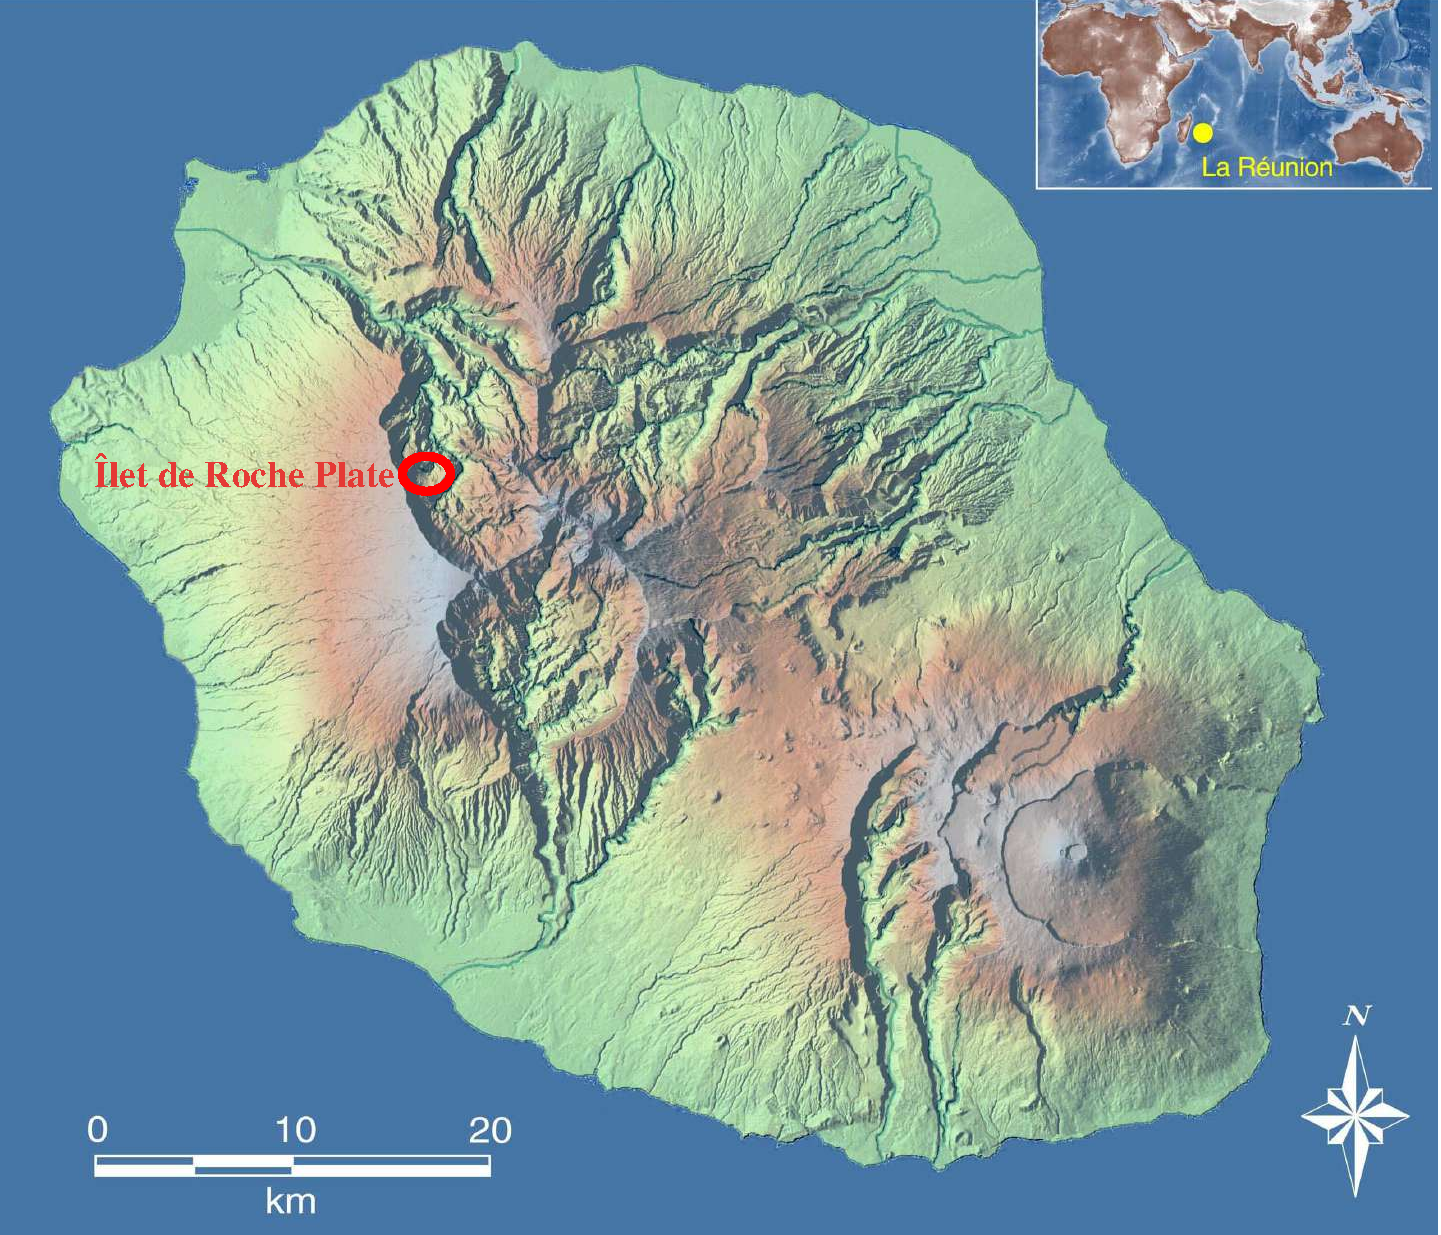
\includegraphics[width=0.7\textwidth]{Introduction/Figures/Carte_Réunion_topo.pdf}
    \caption{Carte topologique de l'île de La Réunion illustrant l'isolement de l'îlet de Roche Plate \cite{reunion_map_commons}}
    \label{fig:topo_reunion}
\end{figure}
\FloatBarrier

La distribution d'électricité y est assurée par le syndicat intercommunal d'électricité de La Réunion (SIDELEC). Historiquement, la production d'énergie sur ce site reposait sur l'utilisation de groupes électrogènes alimentés en carburant fossile. Le ravitaillement en pétrole étant réalisé par hélicoptère, cette solution présente des coûts logistiques élevés ainsi qu'un impact environnemental significatif.

Afin de réduire la dépendance aux énergies fossiles et d'améliorer la durabilité du système énergétique local, un micro-réseau basé sur une production photovoltaïque couplée à un stockage par batteries a été déployé et est actuellement en fonctionnement. Cette première étape vers une production locale d'énergie renouvelable permet de limiter l'usage des groupes électrogènes, tout en soulevant de nouvelles problématiques en termes de gestion de l'intermittence et de stockage de l'énergie.

Dans cette continuité, les travaux présentés dans le cadre du projet ANR GENIAL visent à franchir une nouvelle étape en intégrant une chaîne hydrogène au micro-réseau existant. L'objectif est d'augmenter la capacité de stockage à long terme, d'améliorer l'autonomie énergétique du site et de renforcer la résilience du système face aux variations de production et de consommation.

\subsubsection{Production d'électricité par panneaux photovoltaïques}
Dans ce contexte d'isolement, ce sont les panneaux solaires photovoltaïques qui ont été choisis pour la production intermittente de l'électricité.
\paragraph{Contexte \& principes de fonctionnement} \hfill \\
Les panneaux photovoltaïques sont un outil de conversion de l'énergie électromagnétique solaire en énergie électrique utilisable. Leur production dépend donc entièrement de l'ensoleillement et ce n'est donc pas une source d'énergie pilotable. La production d'électricité dépend de nombre de facteurs comme leur surface, leur composition ou encore leur position angulaire. Ils se démocratisent depuis plusieurs décennies et représentent aujourd'hui environ 6\% de la production d'électricité en France \cite{noauthor_be_nodate}. Leur déploiement est généralement local, plutôt sur le toit de bâtiments qu'en centrales au sol, pour une utilisation qui elle peut être au service du réseau principal ou d'une consommation locale.

Un panneau photovoltaïque utilise l'effet photoélectrique pour convertir l'énergie du rayonnement solaire (onde électromagnétique) en un courant électrique. Un panneau photovoltaïque est composé de cellules, qui sont elles-mêmes composées de matériaux semi-conducteurs comme le silicium. Ces cellules servent d'unités élémentaires dans la conversion de l'énergie solaire en énergie électrique. L'interaction entre les photons incidents et les matériaux semi-conducteurs provoque la libération d'électrons, générant ainsi un courant électrique par l'établissement de paires électron-trou (Fig. \ref{photoelec}). 
\begin{figure}[h!]
    \centering
    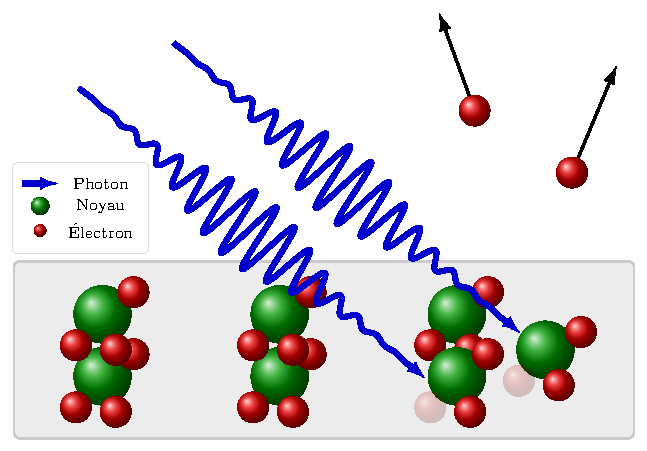
\includegraphics[width=.8\linewidth]{Introduction/Figures/photoelec.pdf}
    \caption{Illustration de l'effet photo-électrique}
    \label{photoelec}
\end{figure}
\FloatBarrier
L'architecture des panneaux solaires repose ensuite sur une disposition interconnectée de ces cellules, configurées en série et en parallèle pour réguler les sorties de tension et de courant. La figure \ref{pola_pv} présente des courbes de polarisation I-V et P-V typiques.
\begin{figure}[h!]
    \centering
    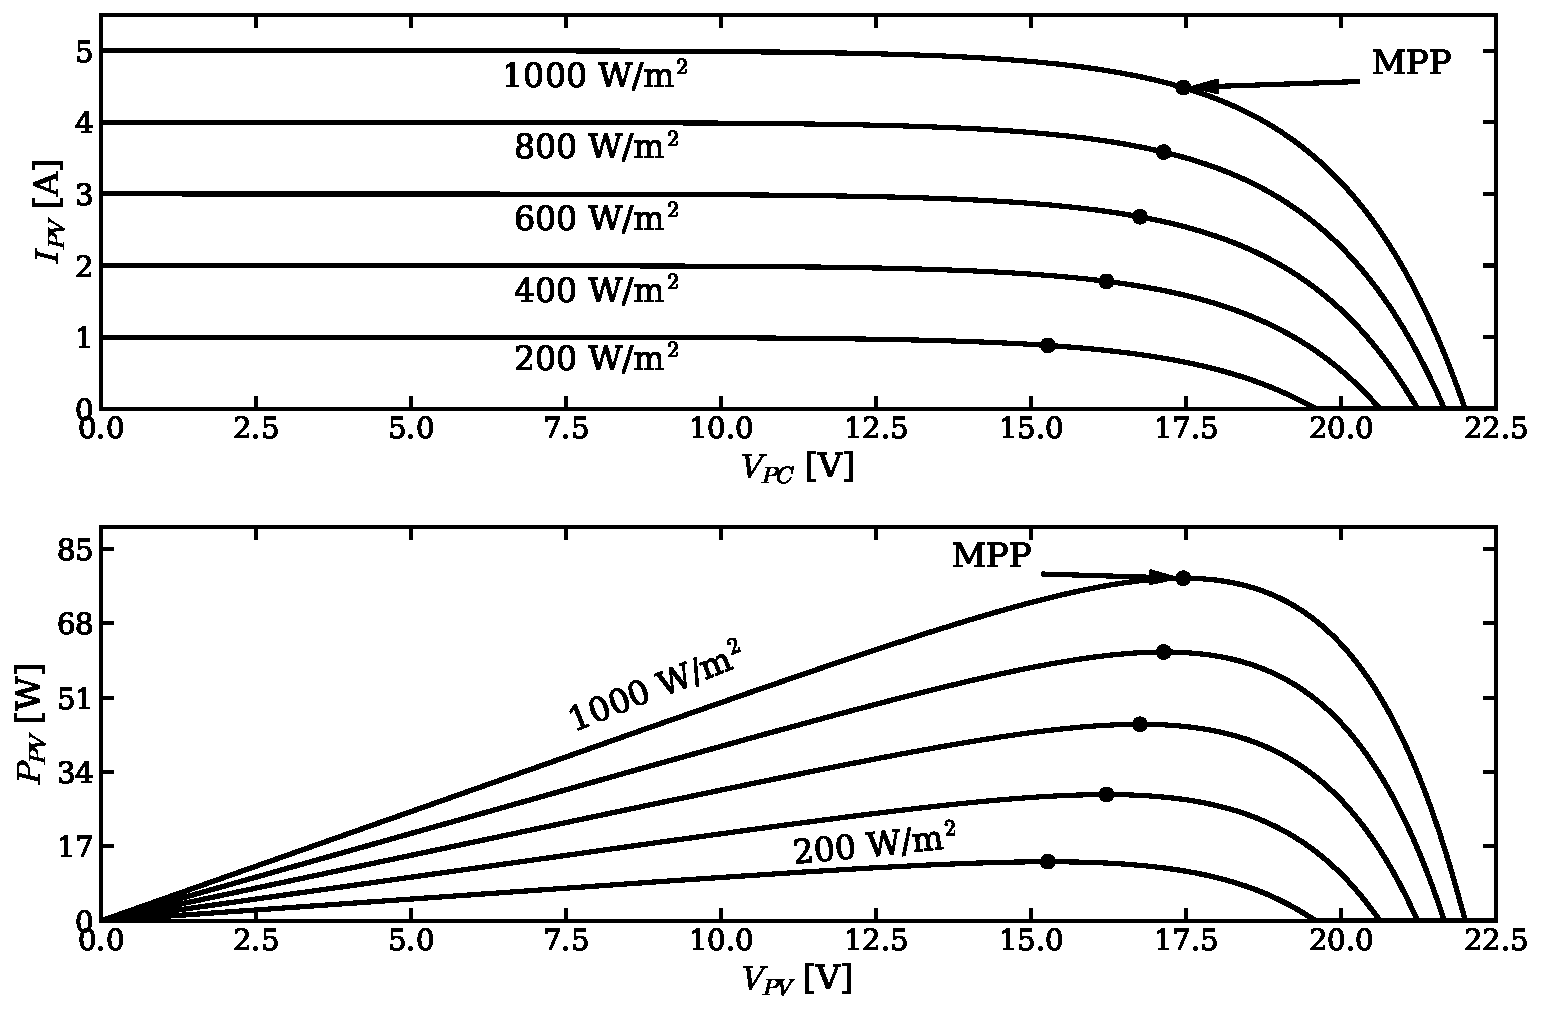
\includegraphics[width=.8\linewidth]{Introduction/Figures/pola-pv.pdf}
    \caption{Courbes de polarisation I-V (haut) et P-V (bas) de panneaux photovoltaïques sous différents niveaux d'irradiance}
    \label{pola_pv}
\end{figure}
\FloatBarrier
Les panneaux photovoltaïques agissant comme une source de courant, il apparaît alors que la puissance fournie dépend grandement de la tension appliquée aux bornes des panneaux. Afin d'obtenir la tension permettant de fournir la puissance maximale, il est commun d'utiliser un algorithme de \textit{Maximum Power Point Tracking (MPPT)} \cite{bayoumi_investigation_2023}\cite{benlahbib_experimental_2020}. Cet algorithme se base souvent sur le principe du \textit{Perturb \& Observe (P\&O)}, où la tension est modifiée de manière monotone en recherchant le point correspondant à la puissance maximale.

\paragraph{Avantages \& Limitations}\hfill \\
Les panneaux photovoltaïques ont donc l'avantage de pouvoir produire de l'énergie électrique de manière renouvelable, en courant continu, et sans émissions directes de gaz à effet de serre. Ils sont également faciles à utiliser à petite échelle et se justifient donc pour des applications décentralisées comme les micro-réseaux. Le défaut majeur des panneaux photovoltaïques réside cependant dans leur forte dépendance aux conditions d'ensoleillement, ce qui ne permet pas de les piloter directement. Ainsi la production de puissance est très variable, et elle est également difficile à prédire avec précision.

\subsection{Généralités sur les batteries}
\subsubsection{Contexte d'utilisation}\hfill \\
Les batteries sont des moyens de stockage de l'énergie électrique sous forme chimique. Elles sont utilisées pour des applications diverses, des appareils électroniques de tous les jours à des banques à grande échelle pour stabiliser le réseau électrique principal \cite{energy_victorian_2023} en passant par des batteries de véhicules électriques, par exemple. Les applications des batteries vont donc de quelques Wh à plusieurs MWh. Dans le cadre de batteries utilisées pour des micro-réseaux électriques, celles-ci trouvent leur place en étant complémentaires des sources de production d'énergie renouvelables intermittentes, comme les panneaux photovoltaïques évoqués plus tôt \cite{molu_optimization-based_2023}\cite{shezan_evaluation_2023}. Les batteries lithium-ion seront à l'étude ici.

\subsubsection{Principes de fonctionnement}\hfill \\
Une batterie lithium-ion fonctionne selon le schéma de la figure \ref{structure_bat}.
\begin{figure}[h!]
    \centering
    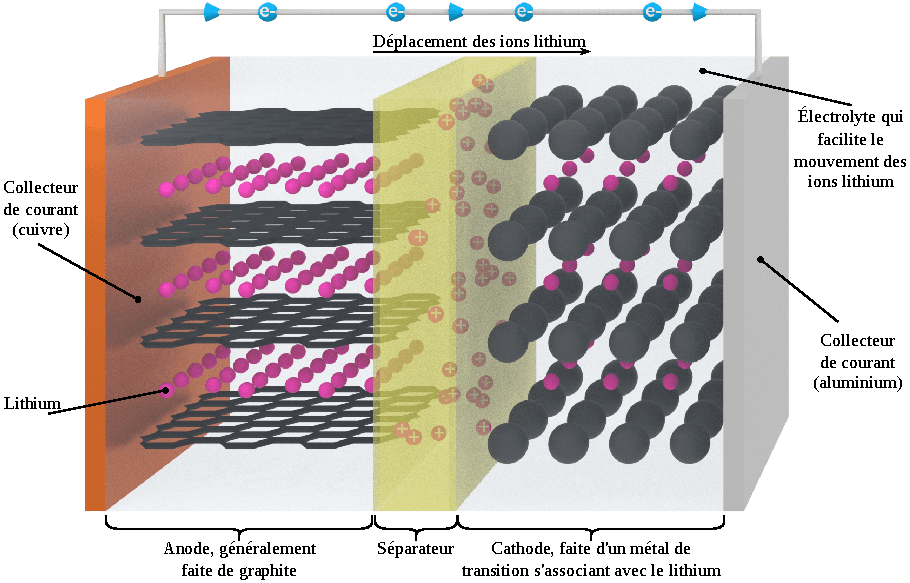
\includegraphics[width=\linewidth]{Introduction/Figures/structure_bat.pdf}
    \caption{Schéma de principe d'une batterie Lithium-ion}
    \label{structure_bat}
\end{figure}
\FloatBarrier

Contrairement à une pile électrochimique classique de type Daniell, une cellule Lithium-ion repose sur des mécanismes d'insertion/extraction d'ions lithium dans des matériaux hôtes, appelés matériaux d'électrode. Il est important que les deux électrodes soient de nature différente car celles-ci jouent des rôles fondamentalement distincts lors des phases de charge et de décharge.

L'anode est généralement constituée de graphite, capable d'insérer des ions lithium dans sa structure (intercalation), tandis que la cathode est constituée d'un oxyde métallique lithié (par exemple LiCoO$_2$, LiMn$_2$O$_4$ ou LiFePO$_4$). Les demi-réactions associées peuvent s'écrire de manière simplifiée comme suit :

\begin{equation}
    x\ce{LiC}_6 \rightleftharpoons x\ce{C}_6 + x\ce{Li}^+ + xe^-
\end{equation}

pour l'anode (graphite) et :

\begin{equation}
    \ce{Li}_{1-x}\ce{MO}_2 + x\ce{Li}^+ + xe^- \rightleftharpoons \ce{LiMO}_2
\end{equation}

pour la cathode (où M représente un métal de transition comme Co, Mn ou Fe).
Chacune de ces électrodes peut être associée à une équation de potentiel de Nernst, dépendant notamment de l'activité des ions lithium dans les matériaux d'insertion. De manière générale, la tension de la cellule dépend de la différence de potentiel électrochimique du lithium entre les deux électrodes.

Contrairement aux piles aqueuses, les cellules Lithium-ion ne comportent pas de pont salin mais un électrolyte liquide (ou polymère) contenant un sel de lithium (typiquement LiPF$_6$), permettant la conduction ionique entre les électrodes tout en empêchant le passage des électrons. Un séparateur microporeux assure également l'isolation électrique entre anode et cathode tout en laissant passer les ions Li$^+$.

Lors d'une décharge, les ions lithium migrent de l'anode vers la cathode à travers l'électrolyte, tandis que les électrons circulent dans le circuit externe, fournissant de l'énergie électrique. Lors de la charge, ce processus est inversé sous l'action d'une source externe
On parle généralement de "cellule" Lithium-ion pour désigner l'unité élémentaire. Ces cellules sont ensuite associées en série et/ou en parallèle pour former des modules, eux-mêmes assemblés en packs, constituant le système final de stockage d'énergie.

\subsubsection{Avantages \& Limitations}\hfill \\
Les batteries sont donc des composants dont les caractéristiques sont très complémentaires de celles des panneaux photovoltaïques, et il est pertinent de les associer dans l'utilisation. Les batteries permettent de stocker de l'énergie électrique de manière relativement durable, en fournissant un courant continu directement utilisable par de nombreuses charges d'aujourd'hui. Les batteries Lithium-ion se distinguent notamment par leur densité énergétique élevée, leur bon rendement et leur faible effet mémoire.

Ces batteries ont cependant le défaut d'être dépendantes de ressources critiques, notamment pour des applications de stockage à grande échelle comme c'est le cas pour de la stabilisation de réseau. Elles sont également très sensibles aux thématiques de vieillissement, et les conditions d'utilisation sont un facteur prépondérant pour l'état de santé d'une batterie. En effet, avec l'utilisation, les batteries voient leur capacité ainsi que leur puissance délivrable diminuer \cite{vetter_ageing_2005}. Il est ensuite vérifié empiriquement que les batteries perdent en capacité avec l'utilisation, celle-ci se dégradant avec le nombre de cycles \cite{ning_cycle_2004}\cite{ning_generalized_2006}.

\subsection{Généralités sur les électrolyseurs}
\subsubsection{Contexte d'utilisation}\hfill \\
Les électrolyseurs, en tant que composants essentiels de la production d'hydrogène par électrolyse de l'eau, suscitent un intérêt croissant dans les stratégies de production d'hydrogène bas-carbone. Leur utilisation s'étend désormais plutôt au secteur stationnaire, où ils facilitent la production d'hydrogène destiné à la génération d'électricité. Cela permet notamment de convertir des surplus d'électricité renouvelable en hydrogène stockable \cite{chatterjee_photovoltaicphoto-electrocatalysis_2022}\cite{brauns_alkaline_2020}. Ils constituent une voie privilégiée de production d'hydrogène bas-carbone lorsqu'ils sont alimentés par une électricité décarbonée. L'hydrogène produit peut avoir plusieurs états, solide liquide ou gazeux, mais la solution la plus répandue est celle de l'hydrogène gazeux sous haute pression. Dans cette section sont décris les électrolyseurs à membrane échangeuse de protons (\textit{Proton Exchange Membrane Water Electrolyzer} (PEMWE)).

\subsubsection{Principes de fonctionnement}\hfill \\
Le principe de fonctionnement d'un électrolyseur repose sur l'application d'un courant électrique à travers une cellule électrolytique, conduisant à la dissociation de l'eau en hydrogène et oxygène.
\begin{figure}[h!]
    \centering
    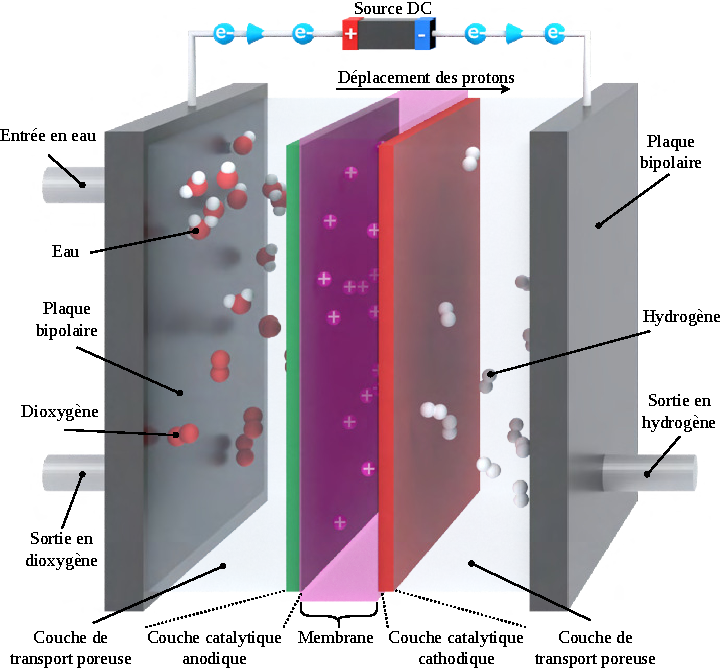
\includegraphics[width=0.7\textwidth]{Introduction/Figures/structure_pemwe2.pdf}
    \caption{Principe de fonctionnement d'un électrolyseur à membrane échangeuse de protons}
    \label{fig:electrolyseur_principe}
\end{figure}
\FloatBarrier
Dans un électrolyseur à membrane échangeuse de protons (PEMWE), la cellule électrochimique est constituée de plusieurs couches fonctionnelles assemblées de manière compacte. On retrouve notamment des plaques bipolaires, des couches de transport poreuses (\textit{Porous Transport Layers}, PTL), des couches catalytiques ainsi qu'une membrane polymère conductrice de protons. L'ensemble membrane--couches catalytiques constitue l'assemblage membrane-électrodes (\textit{Membrane Electrode Assembly}, MEA), cœur actif de l'électrolyseur.
La réaction d'électrolyse de l'eau à l'anode peut être exprimée par l'équation :
\begin{equation}
    \label{eq:anode_electrolyse}
    2\ce{H}_2\ce{O} \rightarrow \ce{O}_2 + 4\ce{H}^+ + 4e^-
\end{equation}
À la cathode, les ions \(H^+\) et les électrons sont réduits pour former de l'hydrogène, selon l'équation :
\begin{equation}
    \label{eq:cathode_electrolyse}
    4\ce{H}^+ + 4e^- \rightarrow 2\ce{H}_2
\end{equation}
Le bilan global de la réaction d'électrolyse de l'eau est représenté par l'équation :
\begin{equation}
    \label{eq:globale_electrolyse}
    2\ce{H}_2\ce{O} \rightarrow 2\ce{H}_2 + \ce{O}_2
\end{equation}
La figure \ref{fig:electrolyseur_principe} illustre le schéma de fonctionnement d'un électrolyseur.

L'eau est injectée du côté anodique de la cellule. Sous l'effet de la tension appliquée, les molécules d'eau sont oxydées au niveau de la couche catalytique anodique, produisant de l'oxygène, des protons et des électrons. Les électrons sont collectés par les couches conductrices puis circulent dans le circuit externe, tandis que les protons traversent la membrane pour rejoindre la cathode.

La membrane est généralement constituée d'un polymère comme que le Nafion\textsuperscript{\textregistered}. Cette membrane assure plusieurs fonctions essentielles : elle permet la conduction protonique entre les deux électrodes, empêche le passage des électrons afin d'éviter le court-circuit interne, et limite le mélange des gaz produits. 

De part et d'autre de la membrane se trouvent les couches catalytiques, constituées de particules catalytiques dispersées dans un ionomère conducteur de protons. En raison de la cinétique lente de la réaction de dégagement d'oxygène, la couche catalytique anodique utilise généralement des métaux nobles à base d'iridium ou de ruthénium (IrO$_2$, RuO$_2$). À la cathode, où la réaction de dégagement d'hydrogène est plus rapide, du platine est généralement employé comme catalyseur.

Les couches de transport poreuses, situées entre les couches catalytiques et les plaques bipolaires, assurent quant à elles plusieurs fonctions de transport. Elles permettent l'acheminement de l'eau vers les sites réactionnels, l'évacuation des gaz produits, ainsi que la conduction électrique et thermique au sein de la cellule. Ces couches sont généralement constituées de matériaux poreux conducteurs. 

Une cellule élémentaire PEMWE fonctionne typiquement sous des tensions comprises entre \(1.8\) et \(2.2\) V selon les conditions opératoires. Comme dans le cas des batteries, plusieurs cellules peuvent ensuite être assemblées en série au sein d'un empilement (\textit{stack}) afin d'augmenter la puissance et la capacité de production d'hydrogène du système.

\subsubsection{Avantages \& Limitations}\hfill \\
L'avantage principal des électrolyseurs réside dans leur capacité à produire de l'hydrogène bas-carbone en utilisant de l'électricité générée à partir de sources renouvelable. Cela contribuant ainsi à l'intégration de ces sources intermittentes dans le réseau. De plus, les électrolyseurs offrent une grande flexibilité en termes de taille et de capacité, permettant une adaptation aux différentes échelles de puissance.
Cependant, Les coûts associés à la production restent élevés, notamment dus aux matériaux coûteux utilisés dans les électrolyseurs. Les électrolyseurs, tout comme les autres éléments permettant le stockage d'électricité cités plus haut, sont également sujets au vieillissement en fonction des conditions d'utilisation, ce qui se traduit notamment par une surtension et donc des pertes de performances \cite{papakonstantinou_degradation_2020}\cite{weis_impact_2019}.


\subsection{Généralités sur les piles à combustible}
\subsubsection{Contexte d'utilisation}\hfill \\
Les piles à combustible sont des appareils de conversion d'un réactif chimique, souvent de l'hydrogène, en électricité. Ce sont des les systèmes complémentaires des électrolyseurs. Les piles à combustible ont des utilisations diversifiées, tant dans le secteur stationnaire, où elles jouent un rôle croissant dans la génération distribuée d'électricité \cite{okundamiya_size_2021}\cite{zhang_performance_2014}, que dans le domaine de la mobilité, où les véhicules à hydrogène alimentés par des piles à combustible offrent dans certains contextes une alternative prometteuse aux moteurs à combustion interne à combustible fossile \cite{chiu_bidirectional_2006}\cite{cipollone_model_2014}. Dans cette section sont décris les piles à combustible à membrane échangeuse de protons (\textit{Proton Exchange Membrane Fuel Cell} (PEMFC)).

\subsubsection{Principes de fonctionnement}\hfill \\
Une pile à combustible est composée de plusieurs éléments clés qui fonctionnent conjointement pour convertir l'énergie chimique en électricité. La structure fondamentale comprend deux électrodes, l'anode et la cathode, séparées par une membrane d'échange de protons (Fig. \ref{fig:pile_structure}). 
\begin{figure}[h!]
    \centering
    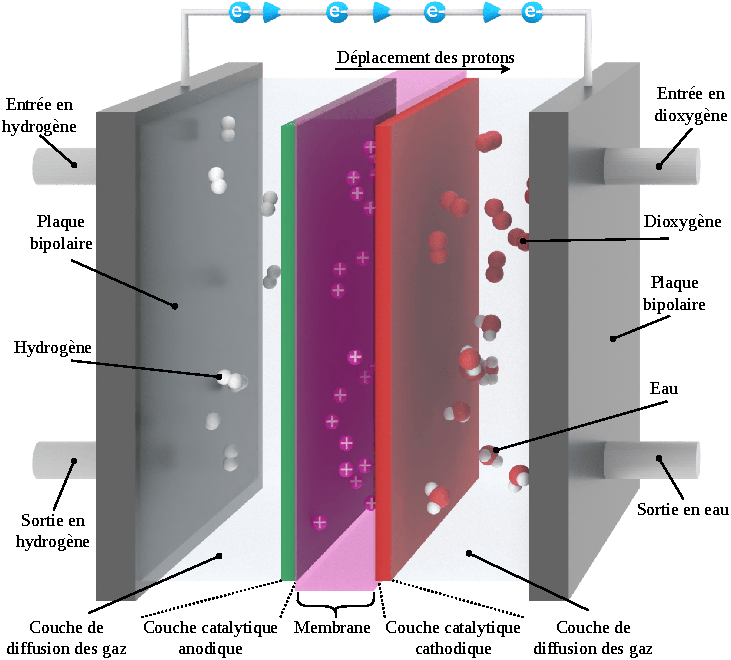
\includegraphics[width=0.7\textwidth]{Introduction/Figures/structure_pemfc.pdf}
    \caption{Structure schématique d'une pile à combustible à membrane échangeuse de protons}
    \label{fig:pile_structure}
\end{figure}
\FloatBarrier
L'hydrogène est injecté à l'anode tandis que l'oxygène, généralement issu de l'air ambiant, est injecté à la cathode. À l'anode, l'hydrogène est oxydé selon la réaction :

\begin{equation}
    \label{eq:anode}
    2\ce{H}_2 \rightarrow 4\ce{H}^+ + 4e^-
\end{equation}

Les protons traversent ensuite la membrane polymère conductrice de protons, généralement à base de Nafion\textsuperscript{\textregistered}, tandis que les électrons circulent dans le circuit électrique externe, produisant ainsi une puissance électrique exploitable.

À la cathode, l'oxygène réagit avec les protons et les électrons pour former de l'eau selon la réaction :

\begin{equation}
    \label{eq:cathode}
    \ce{O}_2 + 4\ce{H}^+ + 4e^- \rightarrow 2\ce{H}_2\ce{O}
\end{equation}

Le bilan global de la réaction est alors :

\begin{equation}
    \label{eq:globale}
    2\ce{H}_2 + \ce{O}_2 \rightarrow 2\ce{H}_2\ce{O}
\end{equation}

Comme pour les électrolyseurs PEM, les couches catalytiques sont constituées de particules catalytiques dispersées dans un ionomère proton-conducteur. Le platine est généralement utilisé comme catalyseur aux deux électrodes, notamment afin d'accélérer les réactions d'oxydation de l'hydrogène et de réduction de l'oxygène. 

Les couches de diffusion de gaz (\textit{Gas Diffusion Layer}, GDL) assurent la distribution homogène des réactifs gazeux vers les sites réactionnels, l'évacuation de l'eau produite ainsi que la conduction électrique et thermique. Elles sont souvent constituées de papiers ou tissus de carbone poreux.

Une cellule élémentaire de PEMFC fonctionne typiquement sous des tensions comprises entre \(0.6\) et \(0.8\) V en charge. Comme pour les batteries et les électrolyseurs, plusieurs cellules sont assemblées en série dans un empilement (\textit{stack}) afin d'augmenter la tension et la puissance du système.

La pile à combustible réalise donc une conversion directe de l'énergie chimique de l'hydrogène en énergie électrique. Contrairement à une batterie, elle nécessite un apport continu de réactifs externes pour fonctionner et son fonctionnement n'est pas réversible au sein d'une même cellule.

\subsubsection{Avantages \& Limitations}\hfill \\
Les piles à combustible présentent des avantages significatifs pour les applications stationnaires. Elles fournissent du courant continu de manière pilotable et sans émission directe de gaz à effet de serre. Cependant, des limitations demeurent, notamment des coûts de production élevés, la nécessité d'une infrastructure d'approvisionnement en hydrogène, et la gestion du vieillissement de ces piles qui se dégradent également avec l'utilisation \cite{dubau_review_2014}. 

\section{Vieillissement des composants}
Chacun des composants du micro-réseau électrique à l'étude (batteries, piles à combustible et électrolyseurs) est sujet au vieillissement et donc à la dégradation dans le temps de ses performances. Ce phénomène complexe est intrinsèquement lié aux conditions d'utilisation spécifiques à chaque application, englobant des paramètres tels que la puissance demandée, la température, et la fréquence des cycles. Cette section va présenter les mécanismes de vieillissement à l'\oe uvre dans chacun des composants du micro-réseau.

\subsection{Batterie}
Les mécanismes de vieillissement des batteries peuvent être très variés. En effet, une batterie étant un assemblage complexe de matériaux interagissant mécaniquement, chimiquement ou encore thermiquement, les défauts peuvent apparaître à des endroits très divers. Un seul de ces défauts peut ensuite avoir un impact sur le comportement global de la batterie et la rendre défaillante. Dans cette partie, ces différents mécanismes de vieillissement seront présentés ainsi que des modèles de vieillissement des batteries.
\subsubsection{Vieillissement d'origine physico-chimique}
\paragraph{Passivation de l'anode}\hfill \\
Juste après leur fabrication, les cellules de batteries subissent une première activation lors de leurs premiers cycles de charge/décharge. Cette activation est nécessaire car elle sert à créer la \textit{Solid Electrolyte Interphase} (SEI), qui est une couche intermédiaire d'électrolyte qui se forme sur l'anode par décomposition de cet électrolyte. Cette couche est notamment importante pour la stabilité de l'électrode, en empêchant une décomposition plus poussée de l'électrolyte lors de cycles futurs. Au fur et à mesure des cycles de la batterie, cette SEI va tout de même continuer à s'épaissir en consommant du lithium et à entretenir la passivation de l'anode. Cette passivation se fait notamment au détriment de la capacité de la batterie \cite{he_effect_2013}\cite{edstrom_new_2006}.

\paragraph{Dépôt de lithium mécanique à l'anode}\hfill \\
Le lithium peut être consommé involontairement par l'épaississement de la SEI, mais il peut aussi se déposer directement à l'anode. Ce phénomène a surtout lieu aux températures les plus froides et, dans une moindre mesure, pour des courants élevés \cite{lin_low-temperature_2001}. Ce phénomène apparaît principalement lors des phases de charge. Le dépôt de ce lithium est problématique car il modifie les propriétés de l'interface électrode/électrolyte, et peut ainsi perturber l'équilibre de la batterie ou encore favoriser la formation de la SEI \cite{fleischhammer_interaction_2015}. Ces dépôts de lithium ont ainsi pour effet de diminuer la capacité de la cellule ainsi que d'augmenter sa résistance interne \cite{petzl_lithium_2015}. 

\paragraph{Modification de la surface cathodique}\hfill \\
Les défauts présentés jusque ici se concentraient à l'anode, mais la cathode n'est cependant pas épargnée. Le principe général est que des réactions chimiques ont lieu aux interfaces électrode/électrolyte, et celles-ci peuvent être des décompositions de l'électrolyte, des dissolutions du matériau de l'électrode ou encore des transitions de phase qui perturbent l'équilibre de la structure cristalline de l'électrode \cite{vetter_ageing_2005}. Ces différentes réactions peuvent donc avoir pour effet de baisser le potentiel de l'électrode et donc par extension de réduire la puissance disponible, ou encore de réduire la capacité et augmenter l'impédance équivalente \cite{bettge_voltage_2013}\cite{vetter_ageing_2005}.

\subsubsection{Vieillissement d'origine mécanique}
Le vieillissement étant très multi-factoriel, il peut également avoir des origines mécaniques. Une cellule durant sa vie va effectivement subir des contraintes mécaniques car ses cycles de fonctionnement vont contribuer à modifier son volume, ce qui aura un impact sur les conditions de pression que subit cette cellule. Cette partie vise à en décrire certains des plus communs.
\paragraph{Matière active}\hfill \\
En étudiant une batterie à l'échelle de la matière active, il est visible que cette matière est organisée en réseau cristallin. La structure de ce réseau va fortement impacter les propriétés de la cellule. Dans le cas où le graphite est utilisé pour l'anode par exemple, celui-ci est disposé en couches afin d'accueillir ou de libérer des ions lithium pendant les cycles de charge et décharge. Cependant, ce graphite peut s'exfolier lorsque c'est un solvant non désiré qui vient s'intercaler dans les mailles. Cela engendre une contrainte inadaptée sur le réseau qui peut ainsi se dégrader et donc moins bien accueillir les ions lithium \cite{shi_effect_2017}\cite{vetter_ageing_2005}. Cela a pour effet de réduire la capacité de la cellule. Il est également possible que des nano-fissurations apparaissent sur l'électrode simplement par insertion des ions lithium dans le réseau cristallin. Ce phénomène est localisé à la cathode et a pour effet d'endommager la matière active \cite{hausbrand_fundamental_2015}. Cela peut notamment ensuite éliminer des couches de passivation qui doivent se régénérer, et donc encore une fois consommer du lithium cyclable.

\paragraph{Électrodes}\hfill \\
Ce sont ces contraintes mécaniques à l'échelle du réseau cristallin qui ont ensuite des conséquences sur la structure mécanique de l'électrode. En effet, celles-ci voient leur volume se modifier lors des cycles, sur des ordres de grandeur de 5\% à 10\% pour des anodes en graphite. Elle sera donc amenée se décrépiter légèrement pendant chaque cycle, ce qui logiquement abîme sa structure. On retrouve donc des zones locales où les ions lithium ne peuvent plus s'accrocher ce qui résulte en une perte de matière active utilisable. On observe également qu'avec les cycles et donc avec les expansions/contractions, la SEI ne peut pas être stable ce qui résulte au fur et à mesure des cycles en une SEI qui s'épaissit et augmente donc la résistance équivalente \cite{wu_designing_2012}. Ces mécanismes de vieillissement sont récapitulés dans le tableau \ref{tab:degradation_liion} : 
\begin{table}[htbp]
    \centering
    \caption{Synthèse des mécanismes de dégradation des électrodes de batteries lithium-ion.}
    \label{tab:degradation_liion}
    \small % Taille de police légèrement réduite pour l'ajustement
    \begin{tabularx}{\textwidth}{@{} l p{3.5cm} l L @{}}
        \toprule
        \textbf{Origine} & \textbf{Mécanisme} & \textbf{Siège} & \textbf{Conséquences} \\
        \midrule
        \multirow{6}{1.5cm}{Physico-chimique} & Passivation (épaississement SEI) & Anode & Consommation de lithium cyclable et perte de capacité \cite{he_effect_2013, edstrom_new_2006}. \\
        \cmidrule{2-4}
        & Dépôt de lithium métallique (\textit{plating}) & Anode & Perturbation de l'interface, favorise la SEI. Hausse de résistance interne et baisse de capacité \cite{lin_low-temperature_2001, fleischhammer_interaction_2015, petzl_lithium_2015}. \\
        \cmidrule{2-4}
        & Modifications de surface & Cathode & Dissolution du matériau, transitions de phase et décomposition de l'électrolyte. Hausse d'impédance et baisse de puissance \cite{vetter_ageing_2005, bettge_voltage_2013}. \\
        \midrule
        \multirow{5}{1.5cm}{Mécanique} & Dégradation de la matière active & Anode / Cathode & Exfoliation du graphite (anode) et nano-fissurations (cathode). Perte de capacité et consommation de lithium \cite{shi_effect_2017, vetter_ageing_2005, hausbrand_fundamental_2015}. \\
        \cmidrule{2-4}
        & Fatigue structurelle des électrodes & Anode & Décrépitation due aux variations de volume (5-10\%). Perte de matière active utilisable, instabilité de la SEI et hausse de la résistance équivalente. \\
        \bottomrule
    \end{tabularx}
\end{table}
\FloatBarrier

\subsection{Électrolyseur}
Le PEMWE opère sous des potentiels anodiques élevés et dans un environnement fortement acide et oxydant \cite{carmo_comprehensive_2013}\cite{shirvanian_novel_2020}. Ces conditions particulièrement sévères induisent des mécanismes de dégradation spécifiques qui limitent la durée de vie du système. 

La littérature scientifique et les analyses post-mortem s'accordent à classer ces dégradations en trois catégories principales : physico-chimiques, thermiques et mécaniques. Elles affectent de manière hétérogène l'ensemble des composants de la cellule (membrane, couches catalytiques, couches de transport poreuses et plaques bipolaires) \cite{feng_review_2017}\cite{wallnofer-ogris_review_2024}\cite{norazahar_degradation_2024}.

\subsubsection{Vieillissement d'origine physico-chimique}

Les altérations d'origine physico-chimique constituent la cause majeure de la réduction des performances et de la durée de vie des électrolyseurs PEM. Elles se manifestent par une augmentation des résistances ohmiques et des surtensions d'activation.

\paragraph{Dégradation chimique de la membrane}\hfill \\
La membrane échangeuse de protons, généralement constituée d'un ionomère perfluorosulfoné (PFSA) tel que le Nafion\textsuperscript{\textregistered}, subit des attaques radicalaires progressives. Le phénomène de perméation croisée (crossover) des gaz H$_2$ et O$_2$ engendre la formation de peroxyde d'hydrogène (H$_2$O$_2$). Ce dernier se décompose en radicaux extrêmement réactifs (HO$^\bullet$ et HOO$^\bullet$), une réaction souvent catalysée par la présence d'impuretés métalliques comme les ions ferreux (Fe$^{2+}$) via la réaction de Fenton \cite{chandesris_membrane_2015}\cite{frensch_impact_2019}. Ces radicaux attaquent les chaînes polymères, provoquant un amincissement de la membrane, l'apparition de micro-perforations et une baisse critique de la conductivité protonique \cite{kuhnert_analysis_2023}.

\paragraph{Dégradation des couches catalytiques}\hfill \\
L'anode, siège de la réaction d'évolution de l'oxygène, utilise des catalyseurs à base d'iridium (Ir/IrO$_2$) pour résister aux hauts potentiels. Cependant, sous polarisation intense, l'iridium subit une dissolution électrochimique (formation d'ions Ir$^{3+}$ ou de complexes IrO$_4^{2-}$). Les ions dissous peuvent migrer à travers la membrane et se redéposer de manière inactive, entraînant une perte directe de surface électrochimiquement active \cite{cherevko_oxygen_2016}\cite{papakonstantinou_degradation_2020}.
À la cathode, le catalyseur à base de platine est sujet à des phénomènes de mûrissement d'Ostwald  et d'agglomération, en particulier lors des cycles de marche/arrêt (\textit{start-stop}) et des périodes en circuit ouvert qui favorisent la corrosion du support carboné \cite{dodwell_open-circuit_2021}\cite{rakousky_analysis_2016}.

\paragraph{Passivation des matériaux et contamination}\hfill \\
Afin de résister à la corrosion anodique, les couches de transport poreuses (PTL) et les plaques bipolaires sont préférentiellement constituées de titane. Néanmoins, l'oxydation inévitable de ce matériau forme une couche de passivation (TiO$_2$) isolante. Sans revêtement protecteur adéquat (or, platine), cette passivation accroît de manière drastique la résistance de contact interfaciale  \cite{bystron_enhancing_2018}\cite{prestat_corrosion_2023}. Par ailleurs, le système est sensible à l'empoisonnement : les cations métalliques (Fe, Cu, Ca) issus de l'eau d'alimentation ou de la corrosion des composants viennent saturer les sites d'échange ionique du PFSA, réduisant la mobilité protonique \cite{li_effect_2019}.

\subsubsection{Vieillissement d'origine thermique} 

Le fonctionnement d'un électrolyseur PEM repose sur un équilibre thermique précis. En régime nominal, la chaleur produite par les surtensions cinétiques et l'effet Joule doit être évacuée par le flux d'eau et les plaques bipolaires \cite{wang_proton_2025}. Une température comprise entre 50 et 80°C est idéale pour les performances \cite{bonanno_review_2024}. Cependant, si la chaleur favorise la réaction chimique et le transport des protons, elle accélère aussi fortement la dégradation des composants. Dans de nombreux cas, la température devient un facteur de stress plus pénalisant que la densité de courant elle-même \cite{urbano_accelerated_2024}. 

 \paragraph{Dégradation aux températures extrêmes}\hfill \\ 

Au-delà de 80\textdegree C, la membrane polymère s'assèche et sa dégradation chimique s'accélère \cite{ayers_research_2010}\cite{pan_review_2021}. Pour le Nafion\textsuperscript{\textregistered}, cela commence par la décomposition des groupements acides sulfonates. Ce phénomène provoque un amincissement de la membrane qui s'amplifie de manière exponentielle avec la température \cite{chandesris_membrane_2015, zhao_review_2019}, devenant critique au-delà de 120\textdegree C \cite{bonanno_review_2024}. 

À l'opposé, les températures négatives ($<0$°C) et les démarrages à froid (\textit{cold start}) sont tout aussi redoutables. L'eau présente dans le polymère peut geler en surface \cite{alink_degradation_2008, pahon_impact_2021}. En gelant, l'eau se dilate et génère des pressions mécaniques qui créent des fissures ou des micro-perforations. Cela peut aller jusqu'à décoller le catalyseur des couches de transport poreuses \cite{yan_effect_2006}. À titre d'exemple, des cycles thermiques brutaux (passant de 80\textdegree C à -10\textdegree C) peuvent réduire les performances de la cellule de 2,3\,\% à 0,6~V \cite{cho_effects_2004}. 

\paragraph{Cyclage thermique et régimes transitoires}\hfill \\ 
Les variations rapides de température liées aux changements de régime font travailler les matériaux. Les polymères et les métaux ne se dilatent pas de la même manière, ce qui crée des tensions mécaniques. À terme, ces cycles provoquent des fissures, affinent la membrane et dégradent les contacts entre les couches, augmentant ainsi la résistance électrique \cite{villagra_analysis_2019}. Un écart de température trop marqué entre l'anode et la cathode peut également faire gonfler ou percer la membrane (MEA) \cite{villagra_analysis_2019}. 

Enfin, les phases d'arrêt et de redémarrage aggravent la dégradation chimique. Lors d'un arrêt, la baisse de température facilite le mélange des gaz à travers la membrane, ce qui favorise l'apparition de radicaux et de peroxyde d'hydrogène \cite{fouda-onana_investigation_2016}. Les redémarrages à froid répétés laissent ainsi une trace mesurable sur l'usure chimique de l'électrolyseur \cite{fouda-onana_investigation_2016}.

\subsubsection{Vieillissement d'origine mécanique}

Les sollicitations mécaniques, qu'elles soient liées à l'assemblage ou au fonctionnement en pression, sont souvent à l'origine de défaillances brutales (microfissures, fuites, courts-circuits).

\paragraph{Contraintes de pression et défauts d'assemblage}\hfill \\
L'application d'une pression de serrage inadéquate ou hétérogène lors de l'assemblage du stack est critique. Une compression excessive écrase la porosité des PTL, altérant la perméabilité aux fluides, tandis qu'un sous-serrage augmente la résistance de contact \cite{lapicque_critical_2016}. De plus, le fonctionnement en pression différentielle (cathode souvent pressurisée à $>30$ bars pour l'hydrogène, anode à pression atmosphérique) impose un stress mécanique transversal sur la membrane, favorisant son fluage, sa déformation et l'apparition de micro-perforations \cite{khorasany_mechanical_2015}.

\paragraph{Délamination des interfaces et gestion des gaz}\hfill \\
Les interfaces entre la membrane et les couches catalytiques sont fragilisées par le gonflement hygrothermique cyclique du polymère. Cette fatigue entraîne une délamination progressive, isolant électriquement certaines zones du catalyseur \cite{qin_modeling_2021}. Enfin, à forte densité de courant, la production massive de gaz génère un masquage par les bulles qui obstrue les pores des PTL. Bien que ce phénomène impacte d'abord le transport de masse de façon réversible, l'accumulation de contraintes locales et les défauts d'évacuation hydrique contribuent à la formation de points chauds, liant intrinsèquement dégradation mécanique, thermique et chimique \cite{yuan_bubble_2023}\cite{maier_mass_2022}.

Un résumé des mécanismes de dégradation des PEMWE est donné dans le tableau \ref{tab:sum_deg_pemwe} :
\begin{table}[htbp]
\centering
\caption{Synthèse des mécanismes de dégradation au sein d'un électrolyseur PEM (PEMWE).}
\label{tab:sum_deg_pemwe}
\small
\begin{tabularx}{\textwidth}{@{} l p{3cm} L L @{}}
\toprule
\textbf{Origine} & \textbf{Mécanisme} & \textbf{Description} & \textbf{Conséquences} \\
\midrule

\multirow{9.5}{*}{Physico-chimique} 
& Dégradation de la membrane 
& Attaques radicalaires (\ce{HO^{$\bullet$}}) via la réaction de Fenton (\ce{Fe^{2+}}) et formation de \ce{H2O2}. 
& Amincissement, micro-perforations et baisse de conductivité protonique \cite{chandesris_membrane_2015, kuhnert_analysis_2023}. \\
\cmidrule(lr){2-4}
& Dissolution et agglomération 
& Dissolution de l'Ir (anode) et mûrissement d'Ostwald du Pt (cathode). 
& Perte de surface active (ECSA) et de l'activité catalytique \cite{cherevko_oxygen_2016, rakousky_analysis_2016}. \\
\cmidrule(lr){2-4}
& Passivation et empoisonnement 
& Formation de \ce{TiO2} isolant sur les PTL/BPP en titane et saturation par cations métalliques. 
& Hausse drastique de la résistance de contact (ICR) et baisse de mobilité protonique \cite{bystron_enhancing_2018, li_effect_2019}. \\

\midrule

\multirow{6}{*}{Thermique} 
& Températures extrêmes 
& Décomposition des groupements sulfonates ($>80$\textdegree C) ou gel de l'eau ($<0$\textdegree C). 
& Dégradation exponentielle du polymère ou fissures par expansion volumique de la glace \cite{ayers_research_2010, alink_degradation_2008}. \\
\cmidrule(lr){2-4}
& Cyclage thermique 
& Dilatations différentielles entre composants lors de régimes transitoires. 
& Fatigue mécanique, délamination et hausse des pertes ohmiques \cite{villagra_analysis_2019, fouda-onana_investigation_2016}. \\

\midrule

\multirow{6.5}{*}{Mécanique} 
& Pression et assemblage 
& Serrage hétérogène et stress dû à la pression différentielle ($\ce{H2}$ côté cathode). 
& Écrasement des pores, fluage de la membrane et fuites de gaz \cite{lapicque_critical_2016, khorasany_mechanical_2015}. \\
\cmidrule(lr){2-4}
& Gestion des gaz et interfaces 
& Fatigue hygrothermique (gonflement) et masquage par les bulles de gaz (\textit{bubble masking}). 
& Délamination des interfaces MEA/PTL et formation de points chauds locaux \cite{qin_modeling_2021, yuan_bubble_2023}. \\

\bottomrule
\end{tabularx}
\end{table}
\FloatBarrier

\subsection{Pile à combustible}

Le vieillissement des piles à combustible à membrane échangeuse de protons (PEMFC) résulte également d'une combinaison complexe de phénomènes physico-chimiques, thermiques et mécaniques affectant les différents composants de la cellule. Ces mécanismes conduisent à une diminution de la surface électrochimique active, à une augmentation des résistances internes et aux pertes de transport de masse, se traduisant par une dégradation globale et irréversible des performances \cite{yousfi-steiner_review_2009}\cite{pahon_review_2022}. 

\subsubsection{Dégradation de la couche catalytique}

La couche catalytique, siège des réactions électrochimiques, est soumise à des conditions sévères de potentiel, de pH (milieu acide) et de température, conduisant à plusieurs mécanismes de vieillissement.

\paragraph{Corrosion du support carboné}\mbox{}\\
Le carbone noir, utilisé comme support pour disperser les nanoparticules de platine, est thermodynamiquement instable aux hauts potentiels. Il subit une réaction d'oxydation, particulièrement favorisée par des températures élevées, une forte humidité ou encore de faibles densités de courant \cite{maass_carbon_2008}\cite{zhao_carbon_2021}. La réaction s'écrit de la façon suivante :
$$\ce{C + 2H2O -> CO2 + 4H^+ + 4e^-}$$
De plus, des conditions de fonctionnement anormales, telles que les phases d'arrêt et de redémarrage ou la sous-alimentation locale, provoquent la formation d'un front $\ce{H2/Air}$ à l'anode \cite{ren_degradation_2020}. L'inversion de tension locale qui en résulte force la corrosion du carbone à la cathode pour fournir les protons nécessaires \cite{gerard_oxygen_2010}. Cette corrosion entraîne le détachement des particules de platine, un amincissement de la couche catalytique, une altération de la porosité et une perte de conductivité électrique \cite{wang_pem_2011}.

\paragraph{Dissolution, agglomération et migration du platine}\mbox{}\\
Le platine, bien que noble, subit une dissolution électrochimique significative pour des potentiels cellulaires compris entre 0.65V et 1.1V \cite{wang_pem_2011}\cite{cherevko_durability_2016}. Les atomes de platine dissous peuvent migrer et précipiter dans la membrane, ce qui réduit la surface active et peut catalyser la formation de radicaux libres \cite{wong_mitigation_2015}. Alternativement, par le phénomène de mûrissement d'Ostwald, les plus petites particules se dissolvent pour se redéposer sur des nanoparticules plus massives, réduisant ainsi le rapport surface/volume et l'activité catalytique globale \cite{meier_design_2014}.

\paragraph{Empoisonnement du catalyseur}\mbox{}\\
Les performances du catalyseur peuvent chuter drastiquement en présence d'impuretés dans les gaz réactifs, principalement issues du reformage des hydrocarbures à l'anode ou de la pollution de l'air à la cathode \cite{zamel_effect_2011}. Le monoxyde de carbone s'adsorbe fortement sur les sites actifs du platine, bloquant l'oxydation de l'hydrogène. Cet empoisonnement est réversible à hauts potentiels via l'oxydation du $\ce{CO}$ en $\ce{CO2}$ \cite{valdes-lopez_carbon_2020}. À l'inverse, le sulfure d'hydrogène ($\ce{H2S}$) provoque un empoisonnement cumulatif avec des pertes d'activité catalytique le plus souvent irréversibles \cite{sethuraman_analysis_2010}. L'ammoniac ($\ce{NH3}$) réagit quant à lui avec les protons pour former des ions ammonium ($\ce{NH4^+}$), diminuant sévèrement la conductivité de la membrane et impactant les performances globales de la cellule \cite{zhao_reviews_2020}.

\subsubsection{Dégradation de la membrane échangeuse de protons}

La membrane, généralement en Nafion\textsuperscript{\textregistered}, assure la conduction protonique et la séparation étanche des gaz. Son vieillissement limite directement la durée de vie du système.

\paragraph{Dégradations chimiques}\mbox{}\\
La dégradation chimique majeure provient des attaques par les radicaux libres (tels que $\ce{HO^{\bullet}}$ et $\ce{HO2^{\bullet}}$). Le peroxyde d'hydrogène ($\ce{H2O2}$), formé comme produit secondaire de la réduction de l'oxygène, réagit avec des ions métalliques contaminants (comme $\ce{Fe^{2+}}$ ou $\ce{Cu^{2+}}$, issus de la corrosion des plaques bipolaires) selon le mécanisme de Fenton pour former ces radicaux extrêmement réactifs \cite{wong_mitigation_2015}\cite{chandesris_membrane_2017}. Ces radicaux attaquent les chaînes latérales hydrophiles et la chaîne principale du polymère, provoquant une dépolymérisation mesurable par le rejet d'ions fluorure ($\ce{F^-}$) dans l'eau produite \cite{wong_macroscopic_2014}. Ce processus entraîne un amincissement de la membrane, augmentant sa perméabilité aux gaz, ce qui nourrit un cercle vicieux de dégradation \cite{wong_mitigation_2015}.

\paragraph{Dégradations mécaniques et thermiques}\mbox{}\\
Le Nafion\textsuperscript{\textregistered} \ se gonfle lorsqu'il est hydraté et se rétracte en s'asséchant \cite{lim_membrane_2014}. Les cyclages hygrothermiques (variations de température et d'humidité relative) imposent des contraintes mécaniques répétées, favorisant la création de micro-fissures et de trous \cite{banan_combined_2015}. Thermiquement, si les températures locales dépassent la température de transition vitreuse du polymère, due à des points chauds liés à la recombinaison directe $\ce{H2/O2}$, la membrane peut perdre irrémédiablement ses propriétés structurelles \cite{aubry_diagnostic_2022}. Enfin, l'exposition à des températures négatives peut geler l'eau interstitielle, causant des micro-déchirures par expansion volumique \cite{amamou_comprehensive_2016}.

\subsubsection{Dégradation de la couche de diffusion des gaz (GDL)}

La couche de diffusion des gaz, constituée d'un substrat fibreux carboné et traitée avec un agent hydrophobe tel que le PTFE, est essentielle pour la gestion de l'eau et la distribution des réactifs.

\paragraph{Altérations mécaniques et perte d'hydrophobicité}\mbox{}\\
L'érosion induite par les flux de gaz élevés et les attaques radicalaires dégradent progressivement le PTFE \cite{park_review_2015}. Cette perte d'hydrophobicité réduit fortement les capacités d'évacuation de l'eau liquide, augmentant drastiquement la vulnérabilité de la cellule au noyage \cite{pan_gas_2021}. Par ailleurs, des contraintes de serrage (compression) excessives du stack ou des épisodes de gel modifient de manière irréversible la macroporosité de la GDL, augmentant la résistance au transport de matière et favorisant la délamination de ses sous-couches \cite{millichamp_mechanisms_2015}.

\subsubsection{Dégradation des plaques bipolaires}

Dans l'environnement de la pile à combustible (milieu acide, humidité élevée, températures pouvant excéder 80\textdegree C et potentiels variables), les plaques bipolaires métalliques sont particulièrement sujettes à la corrosion \cite{tawfik_metal_2007}. 

La corrosion dissout le métal et libère des ions (tels que $\ce{Fe^{2+}}$), qui migrent vers la membrane et aggravent sa dégradation chimique (mécanisme de Fenton détaillé précédemment) \cite{wang_stainless_2003}. Afin de se protéger, certains métaux forment un film de passivation composé d'oxydes. Si ce film prévient une corrosion plus sévère, il a l'inconvénient d'être un mauvais conducteur électrique, augmentant ainsi considérablement la résistance de contact entre la plaque et la GDL, ce qui détériore les performances globales de la cellule \cite{tawfik_metal_2007}.

Un résumé des différents types de dégradation est donné dans le tableau \ref{tab:sum_deg_pemfc}.
\begin{table}[htbp]
\centering
\caption{Synthèse des mécanismes de dégradation des composants d'une PEMFC.}
\label{tab:sum_deg_pemfc}
\small
\begin{tabularx}{\textwidth}{@{} l p{3cm} L L @{}}
\toprule
\textbf{Composant} & \textbf{Mécanisme} & \textbf{Description} & \textbf{Conséquences} \\
\midrule

\multirow{8.5}{2.2cm}{Couche catalytique} 
& Corrosion du carbone support 
& Oxydation du carbone en \ce{CO2} favorisée par les hauts potentiels et les phases \textit{start-stop}. 
& Détachement du Pt, amincissement de la couche, perte de conductivité \cite{gerard_oxygen_2010}\cite{wang_pem_2011}. \\
\cmidrule(lr){2-4}
& Dégradation du platine 
& Dissolution électrochimique (\ce{Pt^{2+}}) et mûrissement d'Ostwald. 
& Réduction de la surface active et de l'activité catalytique \cite{cherevko_durability_2016}\cite{meier_design_2014}. \\
\cmidrule(lr){2-4}
& Empoisonnement 
& Adsorption d'impuretés (\ce{CO}, \ce{H2S}, \ce{NH3}) sur les sites actifs. 
& Blocage des sites réactionnels, baisse drastique des performances \cite{zamel_effect_2011}\cite{sethuraman_analysis_2010}. \\

\midrule

\multirow{5.5}{2.2cm}{Membrane polymère} 
& Attaque chimique 
& Formation de radicaux libres via le mécanisme de Fenton (\ce{Fe^{2+}}). 
& Dépolymérisation, amincissement et augmentation du \textit{crossover} gazeux \cite{wong_mitigation_2015}\cite{chandesris_membrane_2017}. \\
\cmidrule(lr){2-4}
& Fatigue mécanique et thermique 
& Cycles hygrothermiques (gonflement/retrait) et expansion de l'eau gelée. 
& Apparition de micro-fissures et de trous \cite{lim_membrane_2014}\cite{amamou_comprehensive_2016}. \\

\midrule

GDL 
& Dégradation de l'hydrophobicité 
& Altération mécanique et chimique du traitement PTFE. 
& Mauvaise gestion de l'eau, vulnérabilité au noyage (\textit{flooding}) \cite{park_review_2015}\cite{pan_gas_2021}. \\

\midrule

Plaques bipolaires
& Corrosion et passivation 
& Dissolution métallique et formation d'une couche d'oxydes. 
& Hausse de la résistance de contact et empoisonnement de la membrane (\ce{Fe^{2+}}) \cite{wang_stainless_2003}\cite{tawfik_metal_2007}. \\

\bottomrule
\end{tabularx}
\end{table}
\FloatBarrier


\section{Objectifs de l'étude}
\subsection{Présentation des objectifs de la thèse}

Les sections précédentes ont mis en évidence la complexité des phénomènes de vieillissement affectant les composants de stockage et de conversion d'énergie des micro-réseaux électriques. Ces mécanismes sont fortement dépendants des conditions de fonctionnement et impactent directement les performances, la durée de vie ainsi que la disponibilité du système. 
Les stratégies de gestion d'énergie sont un aspect nécessaire au développement de tout système électrique présentant une hybridation des moyens de stockage, et sont l'outil du choix des points de fonctionnement des composants. 
C'est dans ce contexte que le choix de stratégies de gestion d'énergie prenant en compte le vieillissement devient crucial pour garantir un fonctionnement durable et robuste des micro-réseaux intégrant des batteries et une chaîne hydrogène.

Les travaux présentés dans cette thèse s'inscrivent dans cette problématique et ont pour objectif principal de développer des stratégies de gestion d'énergie s'articulant autour du vieillissement des composants. Cette articulation prendra la forme de la résilience au vieillissement (pour des stratégies qui seront donc réactives à ce vieillissement) ainsi que la volonté de sa réduction (pour des stratégies dites anticipatives). Plus précisément, les contributions de ce travail s'articulent autour des trois axes suivants :

\begin{itemize}
    \item l'étude des méthodes de caractérisation, d'estimation et de pronostic de l'état de santé des batteries, piles à combustible et électrolyseurs afin d'évaluer leur état courant ainsi que leur évolution future. Ce sera ici la première brique dans la direction de stratégies de gestion d'énergie éclairées face au vieillissement des composants ;

    \item la définition d'un cadre méthodologique pour l'évaluation et la conception de stratégies de gestion d'énergie adaptées aux contraintes des micro-réseaux avec stockage hybride. Cette étape permettra de définir les axes d'intérêt pour le développement de stratégies ainsi que le squelette des stratégies utilisées ;

    \item l'intégration des informations relatives à l'état de santé des composants et aux prévisions de fonctionnement du micro-réseau dans les stratégies de gestion d'énergie afin d'améliorer  leurs capacités d'anticipation et leur impact sur le vieillissement.
\end{itemize}

\subsection{Plan du manuscrit}

Le premier chapitre est consacré à l'étude de la gestion de l'état de santé des composants de stockage et de conversion d'énergie. Les batteries et les systèmes hydrogène y sont étudiés séparément afin de prendre en compte leurs spécificités propres. Pour chacun des composants, les notions associées à l'état de santé seront d'abord définies, puis les méthodes d'estimation permettant d'évaluer cet état à un instant donné seront présentées. Enfin, les approches de pronostic destinées à prédire l'évolution future des états de santé sont étudiées.

Le deuxième chapitre porte sur la construction du cadre méthodologique de gestion d'énergie. Les critères et indicateurs de performance nécessaires à l'évaluation des stratégies y sont d'abord définis avant de présenter plusieurs stratégies de gestion d'énergie de référence servant de base aux développements réalisés dans la suite du manuscrit.

Le troisième chapitre permettra d'associer les problématiques de vieillissement aux stratégies de gestion d'énergie précédemment développées. Les informations relatives à l'état de santé des composants y sont intégrées afin de construire des stratégies de gestion d'énergie à résilientes au vieillissement et réduisant celui-ci dans le futur. Ce chapitre intègre également des prévisions des profils de production photovoltaïque et de consommation électrique afin d'améliorer les capacités d'anticipation des stratégies proposées.
\newpage